\section{Second Exercise}
Firstly we have that
\begin{equation}
    R_k = 
    \begin{bmatrix}
        1 & 0\\
        0 & e^{2\pi i / 2^k}
    \end{bmatrix}
\end{equation}
We know from Nielsen \& Chuang that we can decompose a controlled $U$-operation as $U = e^{i\alpha}AXBXC$ where $ABC = \I$. See Fig. \ref{fig:rk} for the circuit decomposition.
\begin{figure}[H]
    \centering
    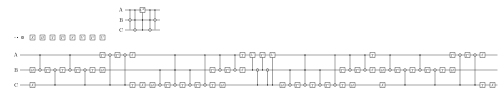
\includegraphics[scale=1.5]{circuit.pdf}
    \caption{Decomposition of $R_k$-operation.}\label{fig:rk}
\end{figure}
Then we have 
\begin{equation}
    R_z(\theta) = 
    \begin{bmatrix}
        e^{-i \theta /2} & 0\\
        0 & e^{i \theta /2}
    \end{bmatrix}
\end{equation}
and the identity $XR_z(\theta)X = R_z(-\theta)$. Thus choosing $\alpha = \pi / 2^k$, $A = \I$, $B = R_z(-\alpha)$ and $C = R_z(\alpha)$ we get
\begin{equation}
    A B C = \I R_z(-\alpha) R_z(\alpha) = R_z(\alpha -\alpha) = R_z(0) = \I
\end{equation}
and
\begin{equation}
    A X B X C = \I X R_z(-\alpha) X R_z(\alpha) = R_z(\alpha)R_z(\alpha) = R_z(2\alpha)
\end{equation}
and finally
\begin{equation}
    e^{i\alpha} R_z(2\alpha) = e^{i\alpha}
    \begin{bmatrix}
        e^{-i\alpha} & 0\\
        0 & e^{i\alpha}
    \end{bmatrix}
    =
    \begin{bmatrix}
        1 & 0\\
        0 & e^{2\alpha i}
    \end{bmatrix}
    =
    \begin{bmatrix}
        1 & 0\\
        0 & e^{2\pi i/ 2^k}
    \end{bmatrix}
    = R_k
\end{equation}